\documentclass[
  11pt,
  letterpaper,
   addpoints,
   answers
  ]{exam}

\usepackage{../exercise-preamble}

\begin{document}

\noindent
\begin{minipage}{0.47\textwidth}

\includegraphics[width=\textwidth]{../fcfm_die}
\end{minipage}
\begin{minipage}{0.53\textwidth}
\begin{center} 
\large\textbf{Electromagnetismo Aplicado} (EL3101-2) \\
\large\textbf{Clase Particular} \\
\small Erik Sáez\\
\end{center}
\end{minipage}

\vspace{0.5cm}
\noindent
\vspace{.85cm}

\begin{questions}
    %%%%%%%%%%%%%%%%%%%%%%%%%%%
    \question Dos barras macizas de cobre de sección rectangular se alinean tal que las caras próximas entre las barras son planas y oblicuas, formando los diferentes ángulos mostrados en la Figura 5 y con una diferencia de potencial $V_0$. Las caras oblicuas son de longitud $L$ y ancho $b$.El espacio entre las caras oblicuas se llena con dos materiales de constantes dieléctricas $\epsilon_1$ y $\epsilon_2$, se debe obtener lo siguiente:
        \begin{enumerate}
            \item Potencial eléctrico $V$ y campo eléctrico $\mathbf{E}$.
            \item Capacitancia para ambas secciones de cobre.
            \item Energía eléctrica $W$ acumulada en ambos medios.
        \end{enumerate}
    \begin{figure}[h!]
        \centering
        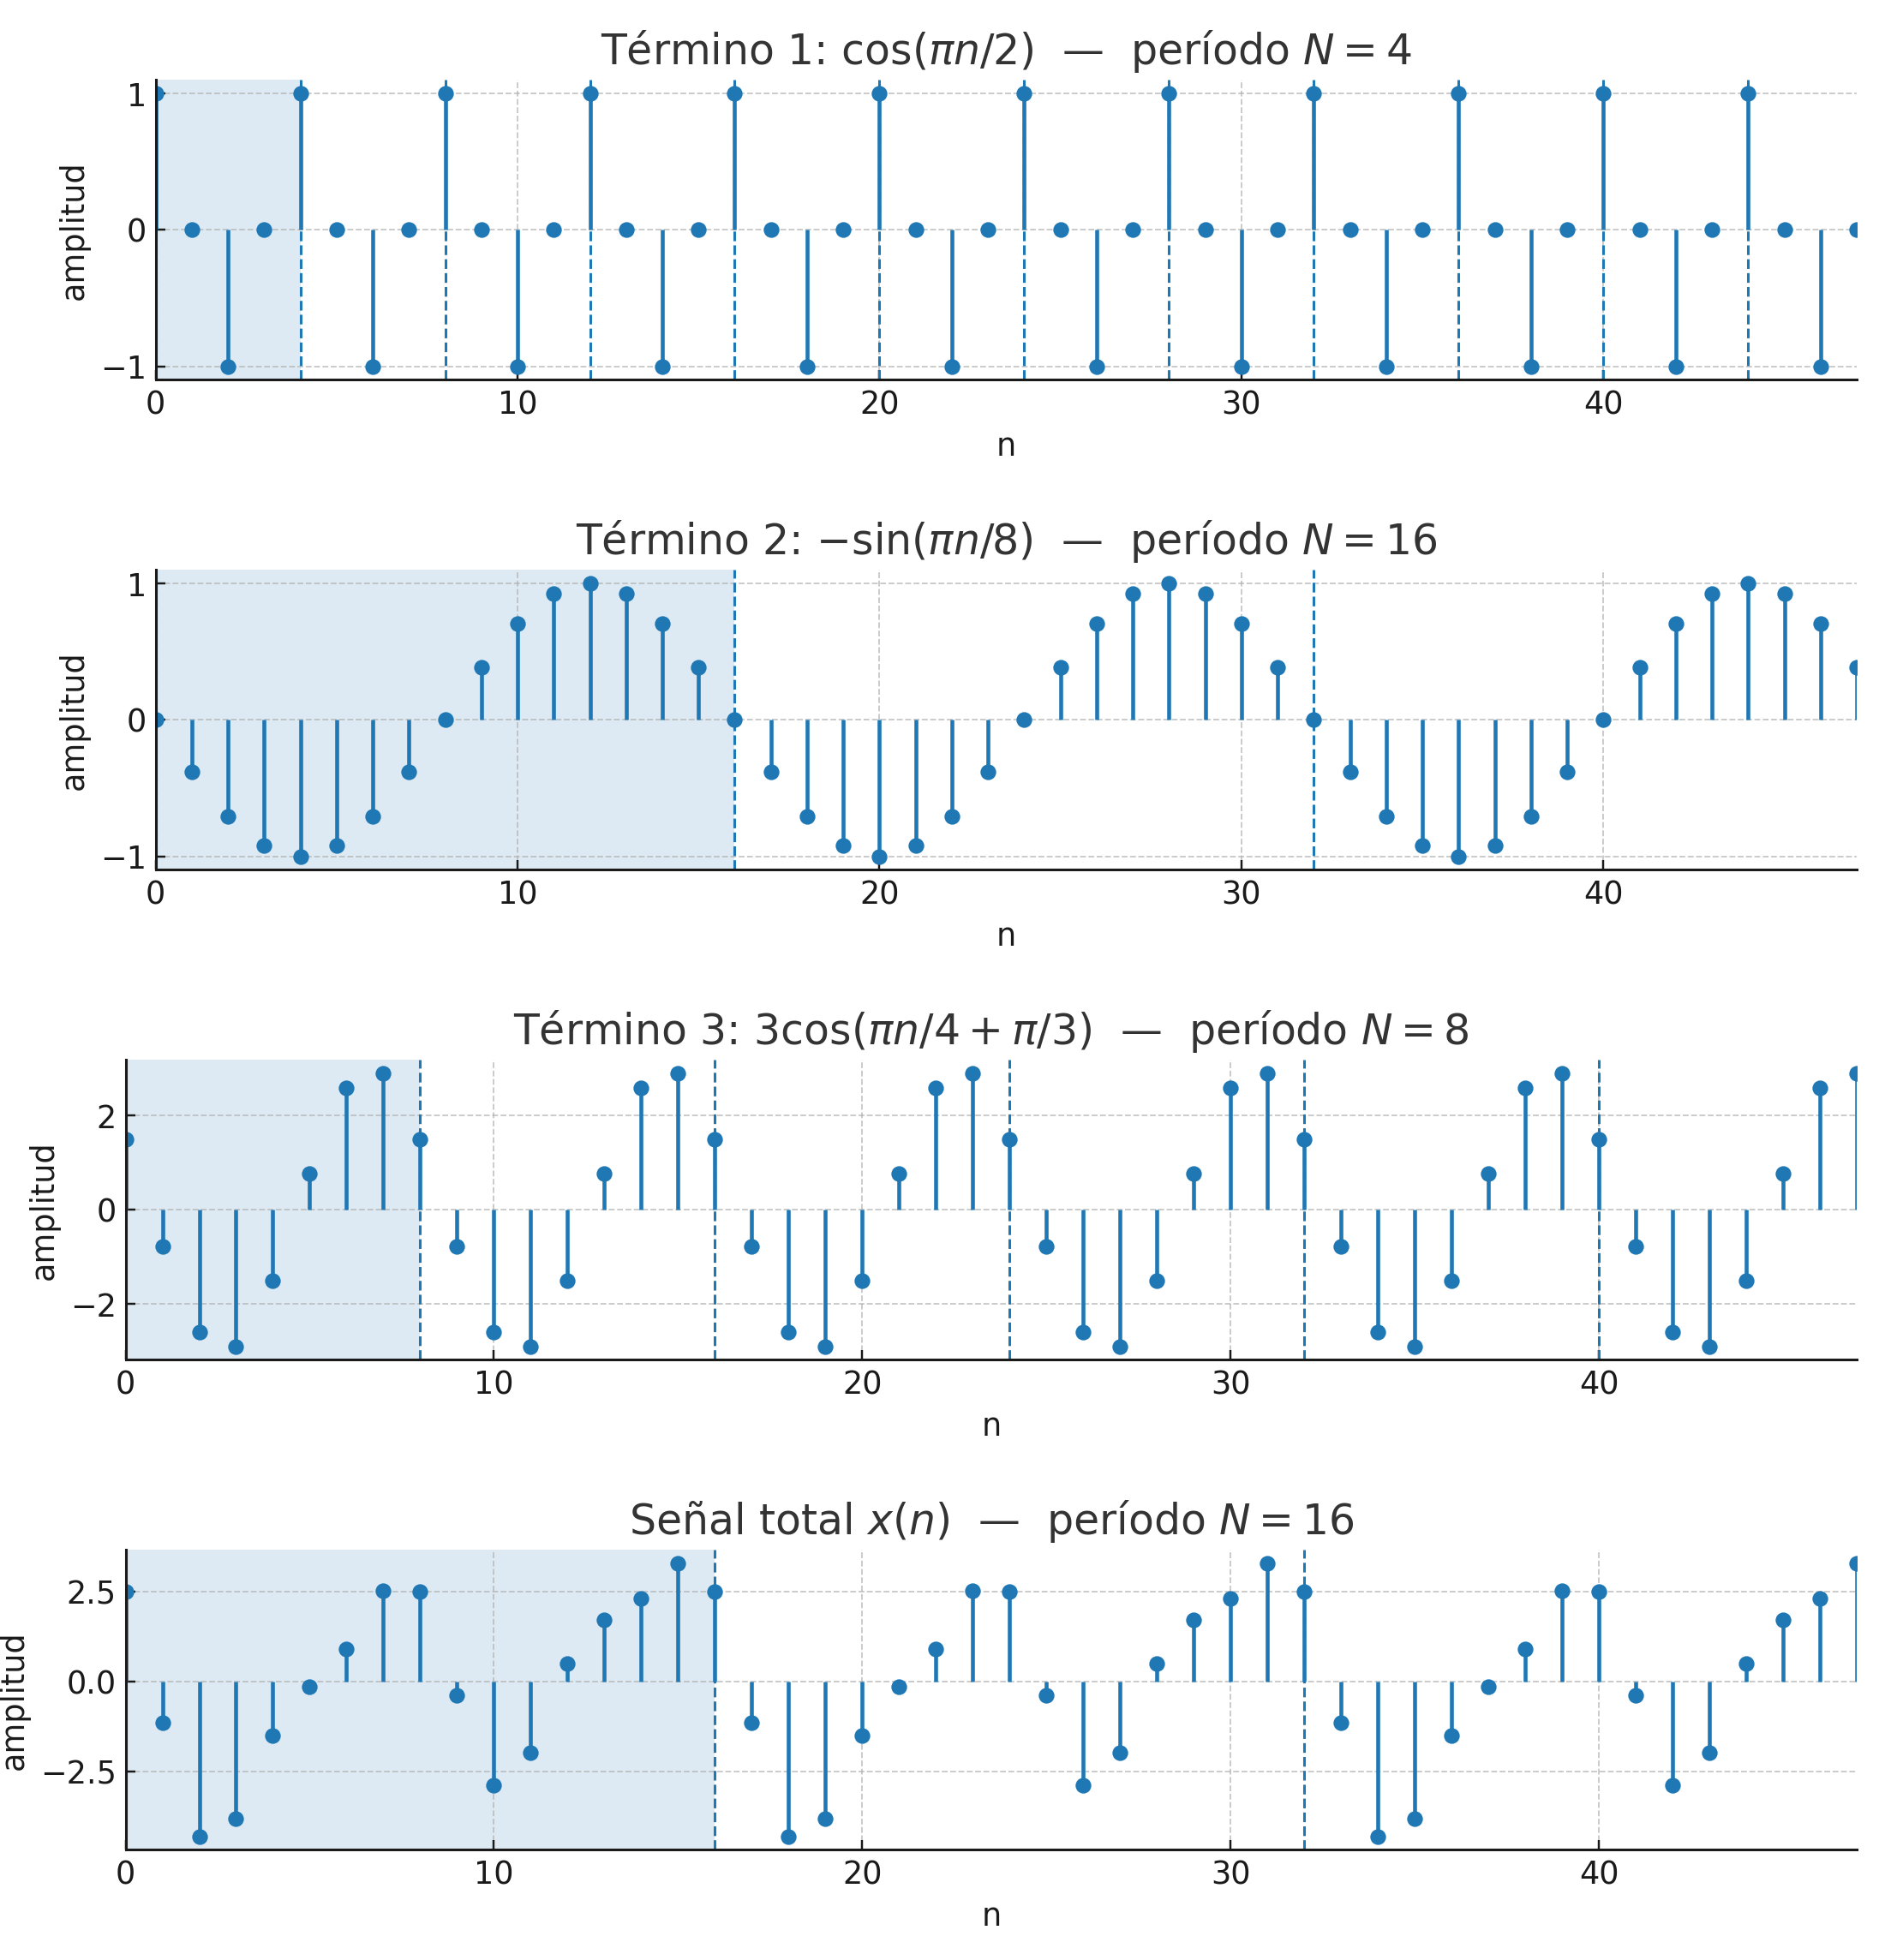
\includegraphics[width=0.7\textwidth]{Auxiliar_1_1}
    \end{figure}
    %%%%%%%%%%%%%%%%%%%%%%%%%%%
   
%%%%%%%%%%%%%%%%%%%%%%%%%%%

\end{questions}
\newpage
%%%%%%%%%%%%%%%%%%%%%%%%%%%

\end{document}